\section{Genetic team composition and level of selection in the evolution of cooperation \cite{waibel2009genetic}}

\begin{frame}{Problem Description}

\begin{figure}
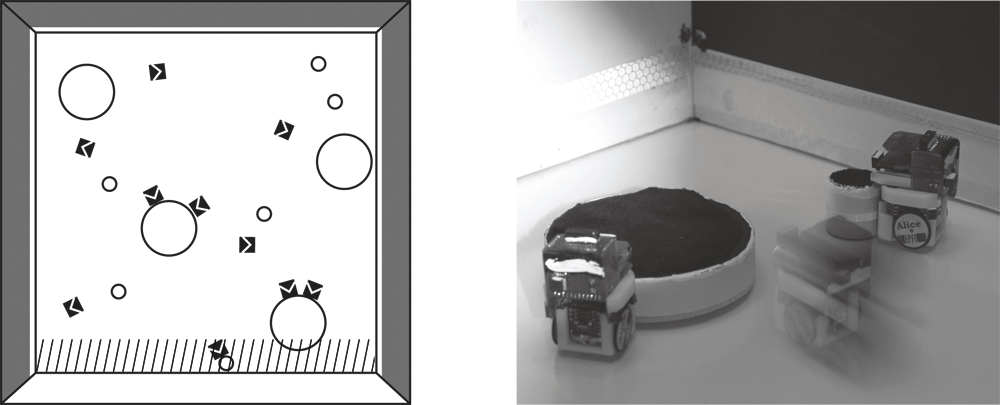
\includegraphics[width=\textwidth]{waibel-fig-3}
\vspace{1ex}
\caption{
Figure 3 from \cite{waibel2009genetic}.
}
\end{figure}

\end{frame}

\begin{frame}{Problem Description}

\textit{Altruistic Cooperative Foraging}
\begin{itemize}
\item six small pucks (1 pt ea to collector)
\item four large pucks (1 pt ea to everybody)
\end{itemize}

\textbf{other tasks:}

\textit{Individual Foraging}
\begin{itemize}
\item six small pucks
\end{itemize}

\textit{Cooperative Foraging}
\begin{itemize}
\item four large pucks
\end{itemize}

\end{frame}


\begin{frame}{Treatments}

\begin{figure}
\begin{columns}
\begin{column}{0.7\textwidth}
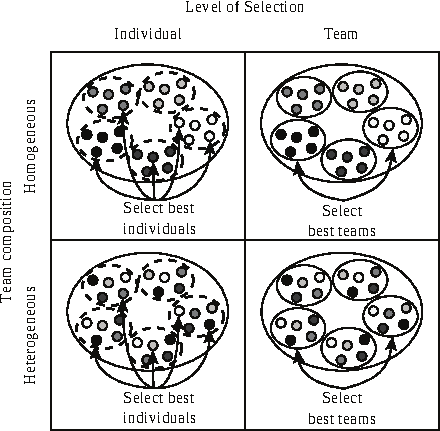
\includegraphics[width=\textwidth]{waibel-fig-2}
\end{column}
\begin{column}{0.3\textwidth}
\caption{
Figure 2 from \cite{waibel2009genetic}.
}
\end{column}
\end{columns}
\end{figure}

\end{frame}

\begin{frame}{Results}

\begin{figure}
\begin{columns}
\begin{column}{0.7\textwidth}
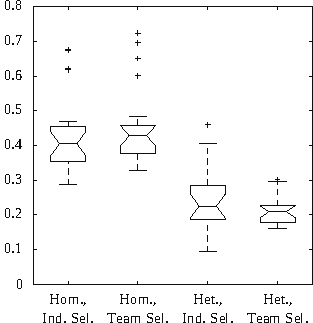
\includegraphics[width=\textwidth]{waibel-fig-9-b}
\end{column}
\begin{column}{0.3\textwidth}
\caption{
Right column of Figure 9 from \cite{waibel2009genetic}.
}
\end{column}
\end{columns}
\end{figure}

\end{frame}

\begin{frame}{Results}


\begin{figure}
\begin{columns}
\begin{column}{0.7\textwidth}
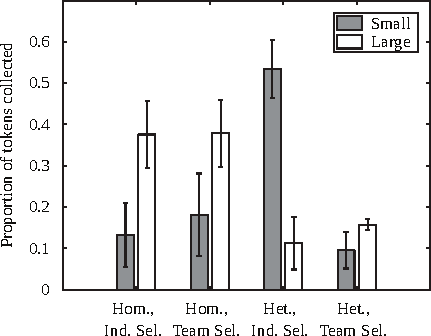
\includegraphics[width=\textwidth]{waibel-fig-10}
\end{column}
\begin{column}{0.3\textwidth}
\caption{
Figure 10 from \cite{waibel2009genetic}.
}
\end{column}
\end{columns}
\end{figure}

\end{frame}

\begin{frame}{Results}

\begin{figure}
\begin{columns}
\begin{column}{0.8\textwidth}
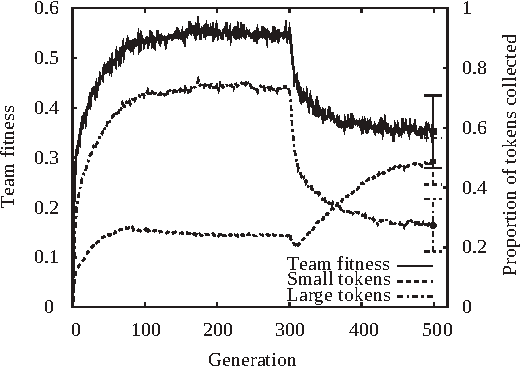
\includegraphics[width=\textwidth]{waibel-fig-12}
\end{column}
\begin{column}{0.2\textwidth}
\caption{
Figure 12 from \cite{waibel2009genetic}.
}
\end{column}
\end{columns}
\end{figure}

\end{frame}

\begin{frame}{Discussion}

directly rewarding large token collection helps address defecting behavior caused by credit-assignment problem under \textit{het., ind. sel}

Figure 12 from \cite{waibel2009genetic} suggests evolutionary contingency not responsible for \textit{het., ind. sel} defecting behavior

weakness: not immediately generalizable to other problem domains
\begin{itemize}
\item e.g., extremely poor performance of local selection treatment in \cite{knudson2010coevolution}
\item requires domain knowledge
\end{itemize}

\end{frame}
